\documentclass[12pt]{article}
\usepackage[czech]{babel}
\usepackage{natbib}
\usepackage{url}
\usepackage[utf8x]{inputenc}
\usepackage{amsmath}
\usepackage{graphicx}
\graphicspath{{images/}}
\usepackage{parskip}
\usepackage{fancyhdr}
\usepackage{vmargin}
\setmarginsrb{3 cm}{2.5 cm}{3 cm}{2.5 cm}{1 cm}{1.5 cm}{1 cm}{1.5 cm}
\usepackage{fancyhdr}
\usepackage{caption}
\usepackage[nottoc,numbib]{tocbibind}
\usepackage[demo]{graphicx}
\usepackage{subfig}
\usepackage{float}
\usepackage{hyperref}
\hypersetup{
    colorlinks=true,
    linkcolor=red,
    filecolor=red,
    urlcolor=blue,
    citecolor=red,
}

\makeatletter
\let\thetitle\@title


\makeatother

\pagestyle{fancy}
\fancyhf{}
\rhead{\theauthor}
\lhead{\thetitle}
\cfoot{\thepage}


%%%%%%%%%%%%%%%%%%%%%%%%%%%%%%%%%%%%%%%%%%%%%%%%%%%%%%%%%%%%%%%%%%%%%%%%%%%%%%%%%%%%%%%%%
\begin{titlepage}
	\centering
	\hspace{1 cm}
    
\includegraphics[scale = 0.35]{FIT_logo.png}\\[1.0 cm]	% University Logo
    \hspace{1 cm}
    \textsc{\LARGE Projektová dokumentace BIN}\\[2.0 cm]
    \hspace{1 cm}
    \textsc{\LARGE Efektivní evoluční návrh\\ \hspace{1 cm} celulárního automatu}\\[0.2 cm]


	\quad\rule{15 cm}{0.2 mm}
	{ \huge \bfseries \thetitle}\\
	
	\vspace{1 cm}
	\begin{minipage}{0.45\textwidth}
		
            \newline
			\emph{Autor:} \\
			\textbf{Tomáš Beránek (xberan46)} \linebreak\\[2.0 cm]
	\end{minipage}\\[0 cm]
	
    \vspace{6 cm}
    \begin{flushleft}
   	    E-mail:\hspace{4 cm}\textbf{xberan46@stud.fit.vutbr.cz} \linebreak
        Datum vytvoření:\hspace{2.1 cm}\textbf{8. května 2022} \linebreak
    \end{flushleft}

	\vfill
    \fancyhf{}
\end{titlepage}

%%%%%%%%%%%%%%%%%%%%%%%%%%%%%%%%%%%%%%%%%%%%%%%%%%%%%%%%%%%%%%%%%%%%%%%%%%%%%%%%%%%%%%%%%

\begin{document}
\afterpage{\cfoot{\thepage }}

\section{Zadání}
Cílem tohoto projektu je návrh a implementace \textbf{efektivního} evolučního algoritmu pro hledání počáteční konfigurace 2D celulárního automatu. Celulární automat se řídí pravidly Game of Life\footnote{Conway's Game of Life -- \url{https://en.wikipedia.org/wiki/Conway\%27s\_Game\_of\_Life}.}. Hledaná počáteční konfigurace musí vést v 1 až N krocích do požadované, předem dané, konfigurace.

\section{Evoluční algoritmus}
Implementovaný EA se řídí běžným schématem:
\begin{itemize}
    \item[1)] náhodná inicializace jedinců
    \item[2)] ohodnocení jedinců
    \item[3)] vybrání rodičů
    \item[4)] křížení rodičů pro získání nových jedinců
    \item[5)] mutace jedinců a skok na 2)
\end{itemize}
Každý \textbf{jedinec} je instance třídy \texttt{GameOfLife}. \textbf{Ohodnocení} každého jedince probíhá zavoláním jeho metody \texttt{makeStep}, která jako argument bere počet kroků, které má CA udělat a vrací \textbf{fitness} -- počet rozdílných buněk mezi hledanou konfigurací a konfigurací jí nejvíce podobnou v průběhu dělání kroků. Fitness je tudíž chyba, kterou se snažíme \textbf{minimalizovat}. 

\textbf{Výběr rodičů} probíhá prahováním -- vybere se pouze N nejlepších jedinců, kteří se stanou rodiči další populace. Počet rodičů je nastavitelným parametrem simulace, viz. kapitola \ref{howtorun}. Bylo experimentováno i s výběrem rodičů podle jejich relativních pořadí, aby se předešlo degradaci populace, ovšem tento způsob naopak ještě zhoršil výsledky experimentů. Nejlepší jedinec každé generace je automaticky a beze změny vybrán do další generace (\textbf{elitismus}). Je využito \textbf{generační EA} -- nová generace je složena pouze z vytvořených potomků (a nejlepšího jedince).

Každý potomek je vytvořen \textbf{křížením} ze dvou náhodně vybraných rodičů. Výstupem každého křížení jsou, kvůli optimalizaci, dva potomci. Na každého takto vygenerovaného potomka je poté aplikována \textbf{mutace}. Veškeré parametry jsou opět nastavitelné.

\subsection{Prostorové genetické operátory}
\textbf{Bodové křížení} je primárně určeno pro křížení vektorů. A i když konfigurace 2D CA je možné reprezentovat jako jediný vektor (takto je také uložen v paměti), tak není vhodné na tuto 2D mapu takto pohlížet. Hlavně z toho důvodu, že při bodovém křížení není možné vybrat např. pouze levou část mapy. Vždy se při bodovém křížení vybere buď pouze část řádku nebo více celých řádků, viz. obrázek \ref{cross}. 

\begin{figure}
    \centering
    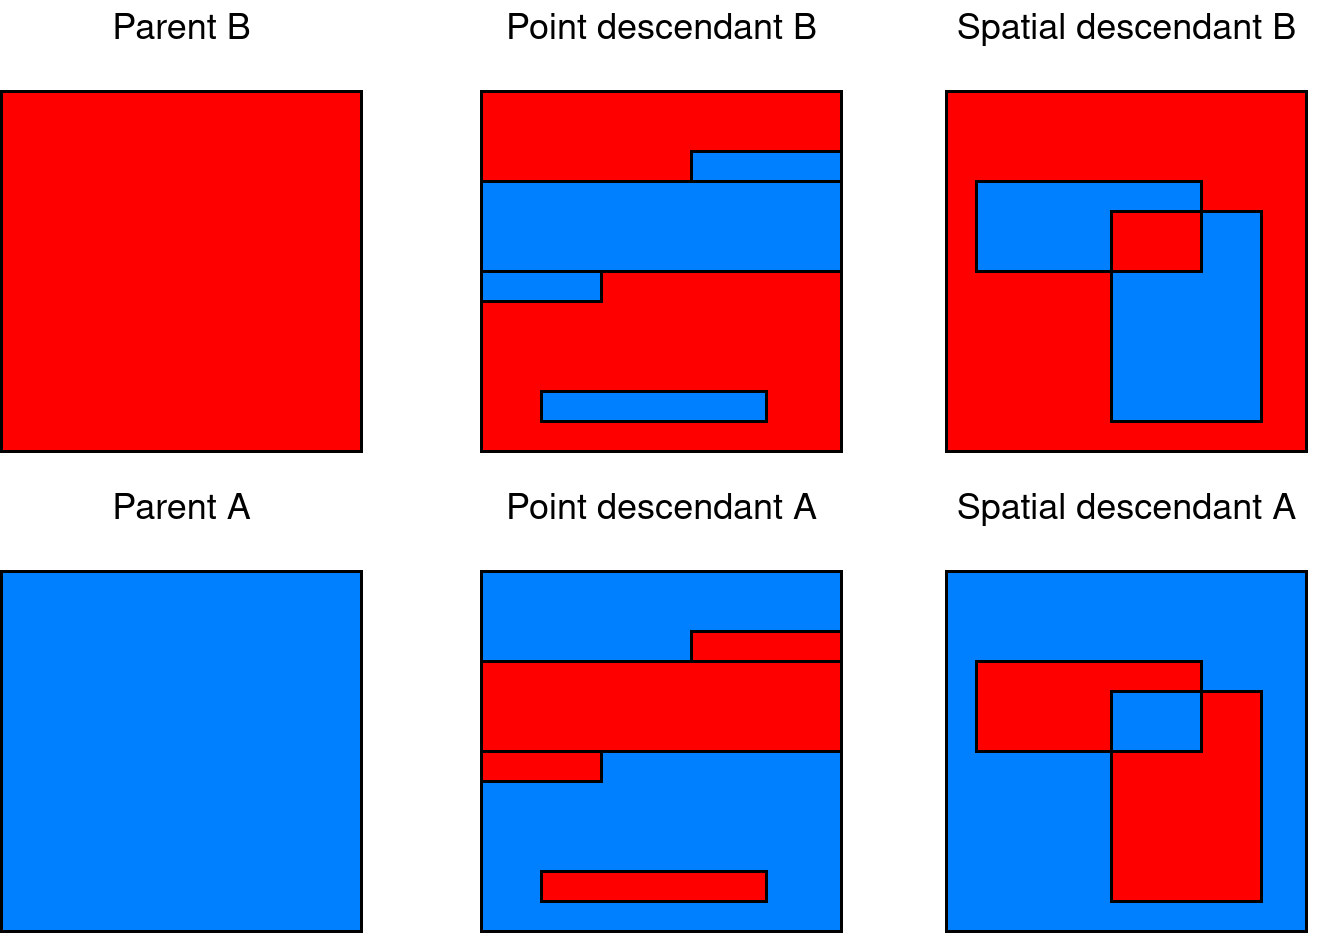
\includegraphics[width=0.6\paperwidth]{cross.png}
    \caption{Porovnání bodového a prostorového křížení.}
    \label{cross}
\end{figure}

\begin{figure}
    \centering
    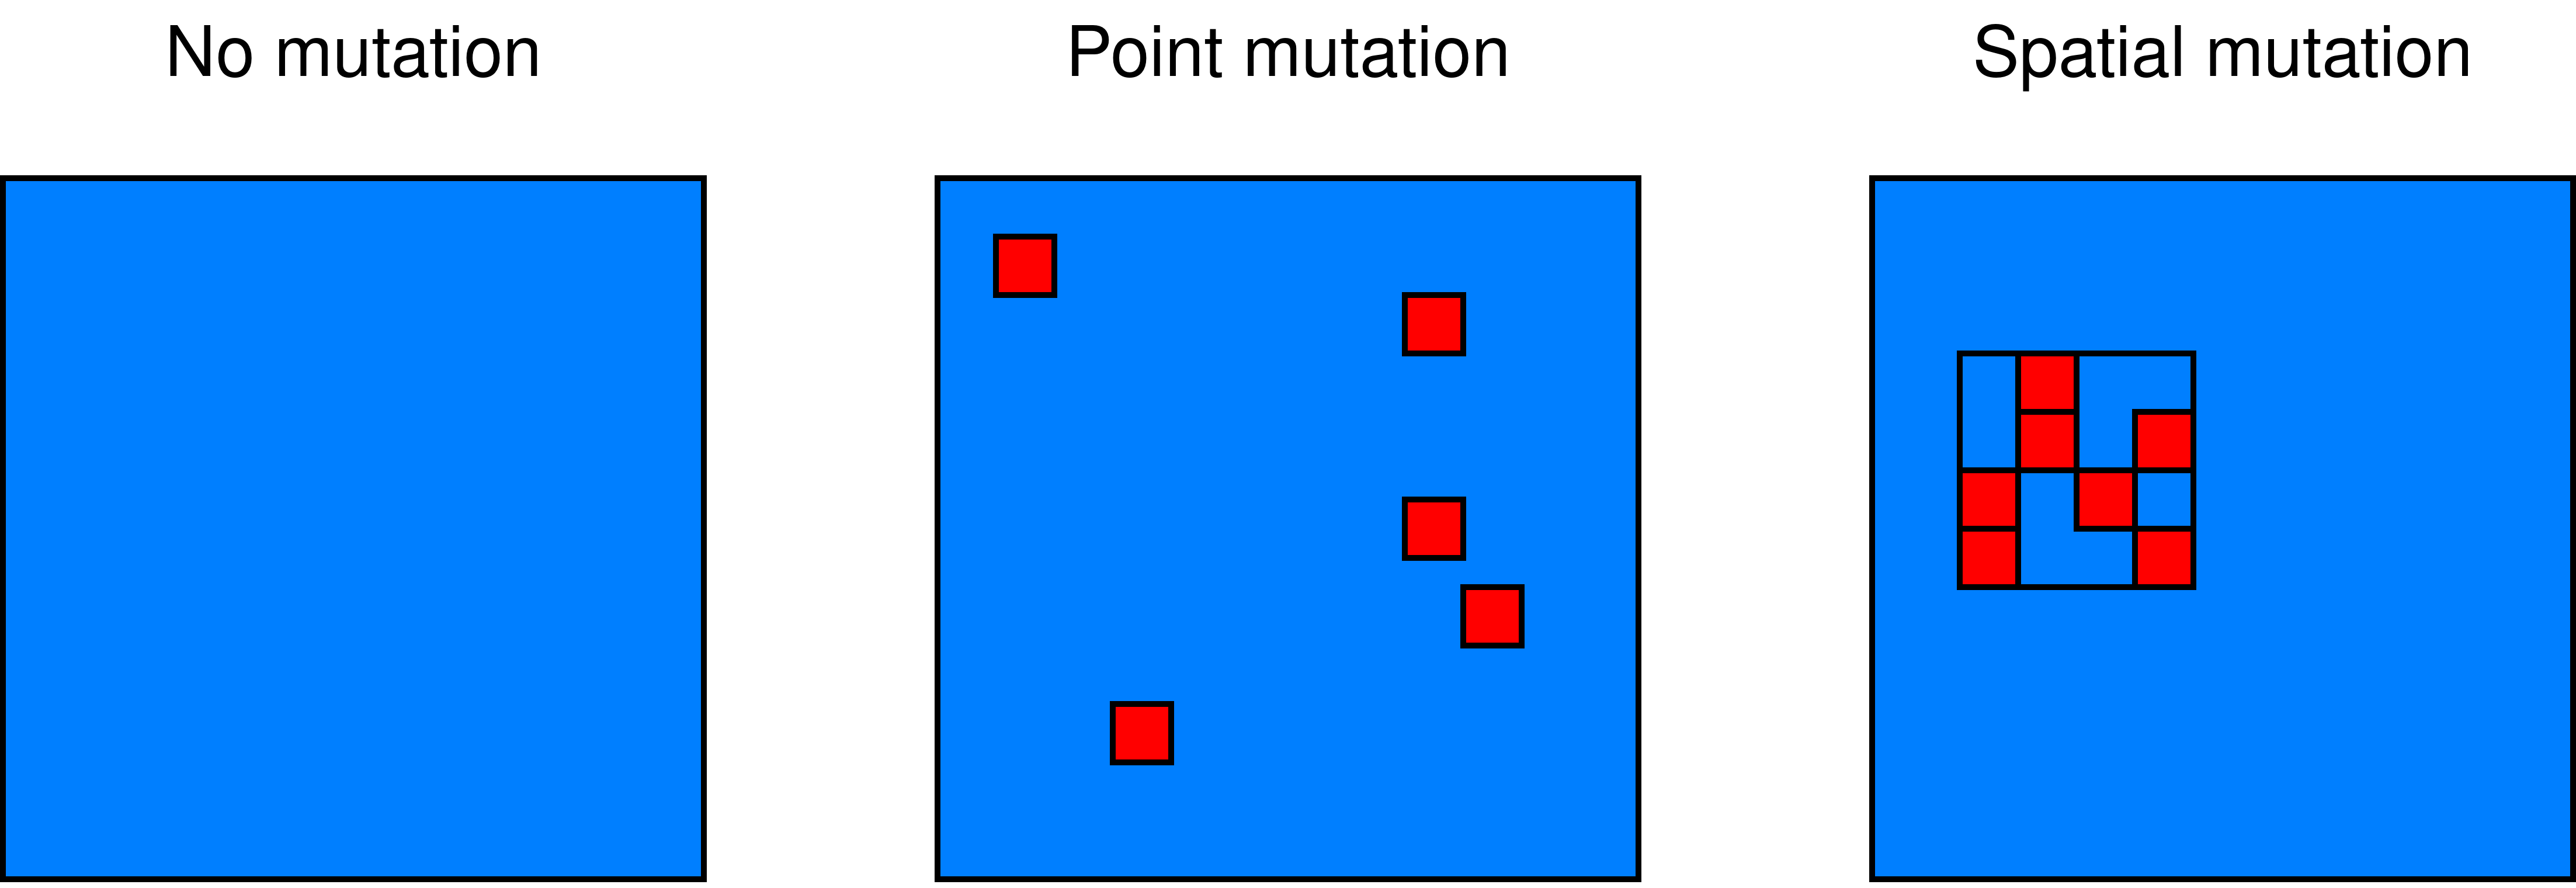
\includegraphics[width=0.6\paperwidth]{mutation.png}
    \caption{Porovnání bodové a prostorové mutace.}
    \label{mutation}
\end{figure}

Z tohoto důvodu bylo navrhnuto a implementováno \textbf{prostorové genetické křížení}, které respektuje 2D povahu Game of Life. Jedná o jednoduché vygenerování náhodného obdélníku, který reprezentuje oblast ve které se vymění informace od obou rodičů. Počet obdélníků je opět nastavitelným parametrem. Pokud se překrývá více obdélníků je jejich efekt podobný negaci, viz. obrázek \ref{cross}.

Vzhledem k povaze pravidel Game of Life není \textbf{bodová mutace} moc úspěšná, protože např. osamocená živá buňka ihned v dalším kroku zemře. Při experimentování jsem narazil na problém vymírání buněk -- EA poměrně rychle zkonvergoval do stavu, kdy byla naprostá většina buněk většiny konfigurací mrtvá a aby bodové mutace dokázaly tyto konfigurace oživit, bylo by nutné jich naakumulovat velké množství a protože jsou tyto mutace rozprostřené, tak při velkém množství už by se EA blížil náhodnému procházení stavového prostoru.

Z tohoto důvodu byla vytvořena \textbf{prostorově koncentrovaná mutace}, která vybere náhodně oblast ve které se s velkou pravděpodobností (např. 50 \%, viz. kapitola~\ref{stat}) znegují stavy buněk. Toto umožní obživnutí určité oblasti mapy. Velikost oblasti byla nastavena na čtverec o ploše 1 \% plochy mapy. Ukázka prostorové mutace je na obrázku \ref{mutation}.

Statistické vyhodnocení bodového a prostorového přístupu je uvedeno v kapitole \ref{stat}.

\section{Optimalizace}
Jedním z hlavním cílů tohoto projektu byla optimalizace EA. Pro měření rychlosti EA byla zvolena metrika \textbf{počet updatů buněk / sekundu}. Počet updatnutých buněk lze vypočítat pomocí vzorce:

\[N_{updates} = G * P * M^2 * S\]

kde G je počet generací, P je velikost populace, M strana čtvercové mapy a S je počet kroků provedených z počáteční konfigurace.

Tato metrika byla zvolena tak, aby byla nebyla ovlivněna např. změnou velikosti mapy (kvůli dobrému zarovnání do cache), atp.

Pro měření času byla použita utilita \texttt{time}. Za hlavní čas byl považován čas strávený v user space. Po implementaci paralelizace se však muselo přejít na real time. Každý čas byl vypočítám jako průměr ze tří spuštění.

\begin{figure}
    \centering
    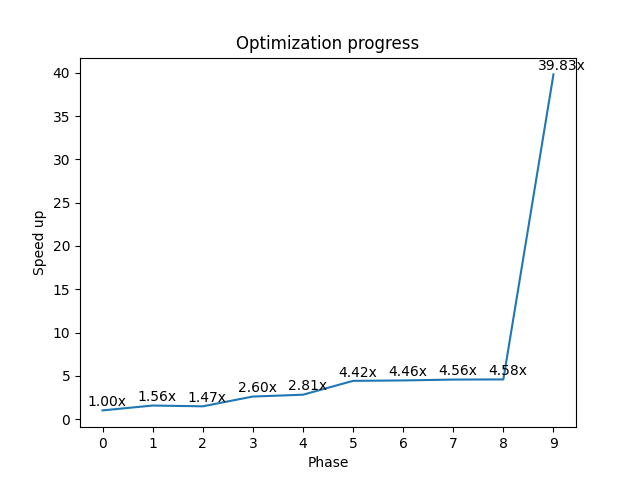
\includegraphics[width=0.6\paperwidth,trim={0  0.2cm 0 0.8cm},clip]{optimization_progress.png}
    \caption{Graf zrychlení jednotlivých úprav.}
    \label{optim}
\end{figure}

\newpage
Optimalizace probíhala v několika fázích, viz. obrázek \ref{optim}. Jednotlivé fáze obsahovaly změny:
\begin{itemize}
    \item[0)] originální řešení -- už zde byla samozřejmě snaha o psaní rozumně rychlého kódu (243 299 u/s)
    \item[1)] zarovnání mapy na 64x64 -- lepší zarovnání v paměti a lepší využití cache (380~090 u/s)
    \item[2)] zpomalení díky přidání prostorových operací (358 114 u/s)
    \item[3)] optimalizace pomocí \texttt{g++ -O1} (632 769 u/s)
    \item[4)] optimalizace pomocí \texttt{g++ -O2} (684 318 u/s)
    \item[5)] optimalizace pomocí \texttt{g++ -O3} (1 074 342 u/s)
    \item[6)] využití rychlejších, ale nepřesných matematických operací (1085623 u/s)
    \item[7)] optimalizace algoritmu -- odebrání zbytečných kopírování polí (1 110 159 u/s)
    \item[8)] přidání \texttt{const} pro lepší informaci pro \texttt{g++} optimalizátor, inlinování funkcí (1~114 071 u/s)
    \item[9)] přidání paralelizace pomocí 12 vláken (9 690 340 u/s)
\end{itemize}


\section{Statistické vyhodnocení}
\label{stat}

Hlavním cílem statistického vyhodnocení bylo \textbf{porovnání bodových a prostorových operací}. Byla provedena sada experimentů s různým nastavením křížení a mutace. Cílem by zjistit, které operace dokáží hledat nejpřesnější řešení. Výsledky experimentů s bodovými operacemi jsou na obrázku \ref{normal}, prostorovými operacemi pro koncentraci mutace 30 \% na obrázku \ref{spatial30}, 50 \% na obrázku \ref{spatial50} a 70 \% na obrázku \ref{spatial70}. Každý bod v grafu udává průměrnou minimální (nejlepší) fitness z 15 běhů na 3 náhodně vygenerovaných hledaných konfiguracích. Hledané konfigurace mají existující řešení, tudíž minimální fitness je 0 a maximální fitness je 4096 (dáno velikostí mapy). Každý běh měl 36 jedinců, 10 rodičů, 500 generací a aplikoval se elitismus.

Z experimentů s \textbf{prostorovými operacemi} lze vidět, že výsledky pro různé procento mutace jsou velmi podobné, nicméně nejlepších výsledků dosahuje mutace 30~\%, viz. obrázek \ref{spatial30}. Konkrétně fitness 825 pro nastavení -- křížení se dvěma obdélníky a koncentrovaná mutace jedné oblasti.

Z experimentů s klasickými \textbf{bodovými operacemi} lze vidět, že nejlepší výsledky jsou pro nízké procento mutací, viz. obrázek \ref{normal}. Také je vidět, že příliš nezáleží na počtu bodů křížení. V průměru dosahují bodové operace lepších výsledků než prostorové, ovšem zdaleka nejlepší fitness je pro prostorové operace -- 825 oproti nejlepší fitness bodových operací -- 832. 

Nejlepší nalezené nastavení je dále použito pro experimenty s \textbf{fixním počtem vyhodnocených fitness} a měnícím se poměrem -- počet generací/velikost populace. Cílem tohoto experimentu je zjistit, zda např. velký počet jedinců a menší počet generací není výhodnější pro tuto úlohu než nízký počet jedinců a mnoho generací.

Výsledky experimentu jsou na obrázku \ref{gen}. Každý bod je průměrem nejlepších fitness z 15 běhů na 3 náhodných konfiguracích. Z grafu lze vyčíst, že pro tuto úlohu je rozhodně \textbf{lepší využívat generace s větším počtem jedinců} (jednotky stovek).

\section{Programovací jazyk a knihovny}
Samotná simulace je napsána v jazyku C++, zejména z důvodu jednoduché paralelizace a velmi dobrého optimalizátoru v \texttt{g++}. Pomocné skripty pro měření, statistické vyhodnocení a vytvoření grafů jsou napsány pro Python3.

Implementace EA byla inspirována kódem prezentovaným na BIN cvičení\footnote{\url{https://github.com/mrazekv/bin-lab-ca/}}. Bylo využíváno standardních knihoven a knihoven \texttt{jsoncpp} a \texttt{pthread} pro C++. Pro Python3 pouze standardních modulů.

\section{Návod na spuštění}
\label{howtorun}
Pro pohodlnější změnu parametrů simulace jsou všechna nastavení uložena v souboru \texttt{config.json} v kořenové složce adresáře. Simulaci je tak možné vyhodnocovat pro různá nastavení bez nutnosti opětovné kompilace. \texttt{config.json} obsahuje:
\begin{itemize}
    \item \textbf{TargetMap} -- soubor s požadovanou konfigurací (jeho formát si lze prohlédnout ve složce \texttt{patterns/})
    \item \textbf{OutputMap} -- výstupní soubor s nejlepším nalezeným řešením
    \item \textbf{MapSize} -- velikost strany čtvercové mapy (cyklické okraje)
    \item \textbf{StepsGOL} -- počet kroků pro každé vyhodnocení fitness
    \item \textbf{Population} -- velikost populace (optimálního výkonu se dosáhne, pokud je velikosti populace dělitelná 12)
    \item \textbf{Elitism} -- informace, zda používat elitismus
    \item \textbf{ParentPopulation} -- počet vybíraných rodičů
    \item \textbf{MaxMutationPercetange} --
       \begin{itemize}
           \item[0] -- žádná mutace
           \item[$>$ 0] -- maximální pravděpodobnost na bodovou mutaci
           \item[$<$ 0] -- maximální počet oblastí pro prostorově koncentrovanou mutaci
       \end{itemize}
    \item \textbf{Generations} -- počet generací
    \item \textbf{Crossover} -- 
       \begin{itemize}
           \item[0] -- uniformní křížení
           \item[$>$ 0] -- počet obdélníků pro prostorové křížení
           \item[$<$ 0] -- počet bodů pro bodové křížení
       \end{itemize}
    \item \textbf{ConcentratedMutation} -- pravděpodobnost na mutaci buňky v oblasti prostorové mutace
\end{itemize}

Pro automatizaci jednotlivých kroků řešení byl napsán \texttt{Makefile} s cíly:
\begin{itemize}
    \item \textbf{run/all} -- spustí vytvořenou binárku simulace s nastavením v \texttt{config.json}
    \item \textbf{compile/install} -- vytvoří binárku simulace
    \item \textbf{clean} -- odstranění dočasných souborů -- včetně defaultního souboru s nejlepším řešením!
    \item \textbf{test} -- vypočítá metriku updates/s pro nově přeloženou simulaci
    \item \textbf{statistics} -- znovu vyhodnotí veškeré experimenty -- výstupem jsou soubory:
       \begin{itemize}
           \item \texttt{statistics.csv} -- výsledky experimentů pro porovnání bodových a prostorových operací
           \item \texttt{statistics2.csv} -- výsledky experimentů pro určení vhodné velikosti populace  
       \end{itemize}
    \item \textbf{graph} -- vytvoření grafů ze souborů \texttt{statistics.csv} a  \texttt{statistics2.csv} a jejich uložení do složky \texttt{graphs/}
\end{itemize}

\section{Závěr}
Cílem tohoto projektu bylo navržení a implementace \textbf{efektivního} EA pro hledání počáteční konfigurace Game of Life. Vylepšení efektivity bylo rozděleno do tří kroků -- zrychlení kódu, vylepšení genetických operací a vyladění hyperparametrů EA. Kód byl zrychlen téměř \textbf{40x} oproti baseline řešení. Pomocí statistického vyhodnocení bylo ukázáno, že nejlepších výsledků dosahují navržené a implementované \textbf{prostorové operátory}. Nejlepší nastavení bylo poté použito pro nalezení vhodné velikosti populace pro tuto úlohu. Ukázalo se, že na náhodně vygenerovaných hledaných konfiguracích je \textbf{nejlepší používat křížení pomocí dvou obdélníků s jedním místem koncentrované mutace} a \textbf{používat vysoké počty} (v řádu stovek) \textbf{jedinců} v každé populaci.

Navržené řešení ovšem není ani zdaleka na vrcholu efektivity. Určitě je možné dále optimalizovat kód i hyperparametry simulace. Pro další optimalizaci kódu by bylo např. možné využít konvoluce pro rychlé počítání živých/mrtvých buněk v okolí a využití GPU pro rychlé provedení konvoluce. Tato úprava by měla velmi velký vliv na zrychlení, protože právě děláním kroků je stráveno 98 \% času simulace (podle nástroje \texttt{valgrind} a \texttt{kcachegrind}). Pro nalezení vhodnějších hyperparametrů by bylo nutné provést více experimentů, ty jsou ovšem časově velmi náročné -- experimenty v této dokumentaci zabraly přibližně 35 hodin na procesoru Intel(R) Core(TM) i5-10400F CPU @ 2.90GHz s 6 jádry a hypertrhreadingem.


\newpage
\begin{figure}
    \centering
    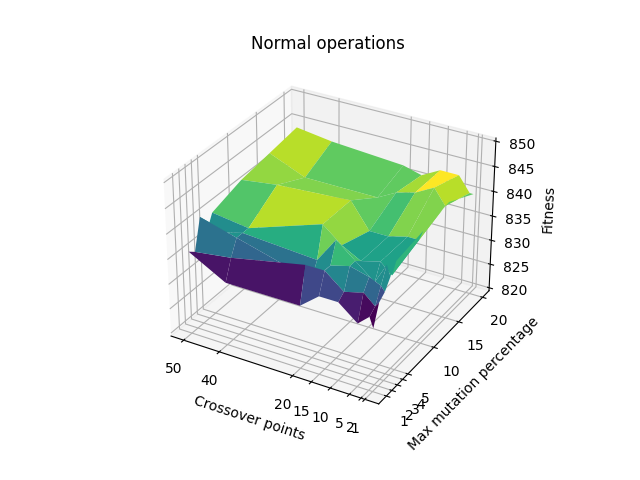
\includegraphics[width=0.6\paperwidth,trim={0  0.cm 0 0.8cm},clip]{normal.png}
    \caption{Výsledky experimentů pro bodové operace.}
    \label{normal}
\end{figure}

\begin{figure}
    \centering
    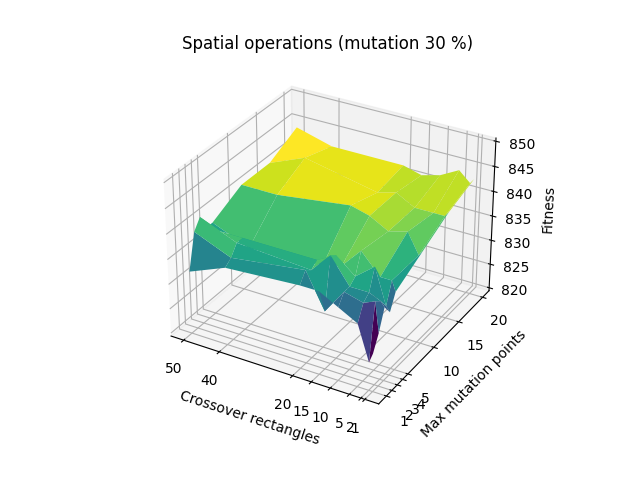
\includegraphics[width=0.6\paperwidth,trim={0  0.2cm 0 0.8cm},clip]{spatial30.png}
    \caption{Výsledky experimentů pro prostorové operace s pravděpodobností na mutaci 30 \%.}
    \label{spatial30}
\end{figure}

\begin{figure}
    \centering
    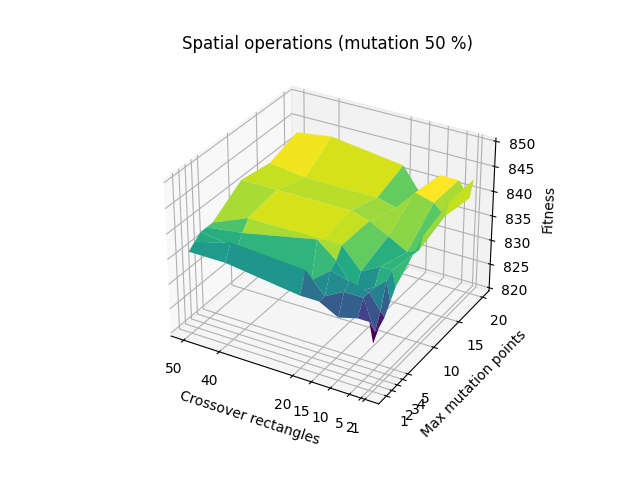
\includegraphics[width=0.6\paperwidth,trim={0 0.2cm 0 0.8cm},clip]{spatial50.png}
    \caption{Výsledky experimentů pro prostorové operace s pravděpodobností na mutaci 50 \%.}
    \label{spatial50}
\end{figure}

\begin{figure}
    \centering
    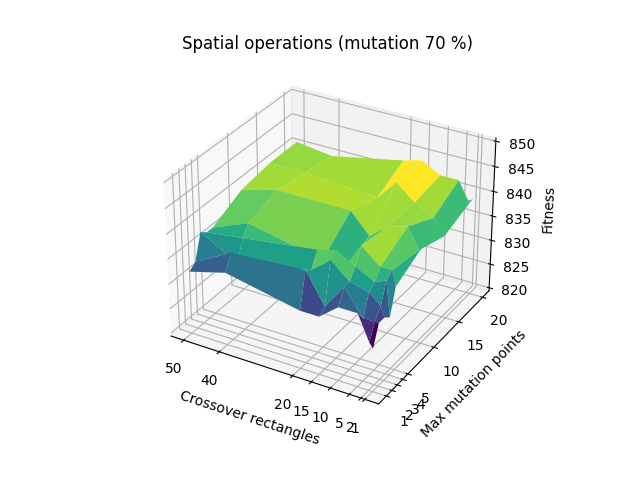
\includegraphics[width=0.6\paperwidth,trim={0  0.2cm 0 0.8cm},clip]{spatial70.png}
    \caption{Výsledky experimentů pro prostorové operace s pravděpodobností na mutaci 70 \%.}
    \label{spatial70}
\end{figure}

\begin{figure}
    \centering
    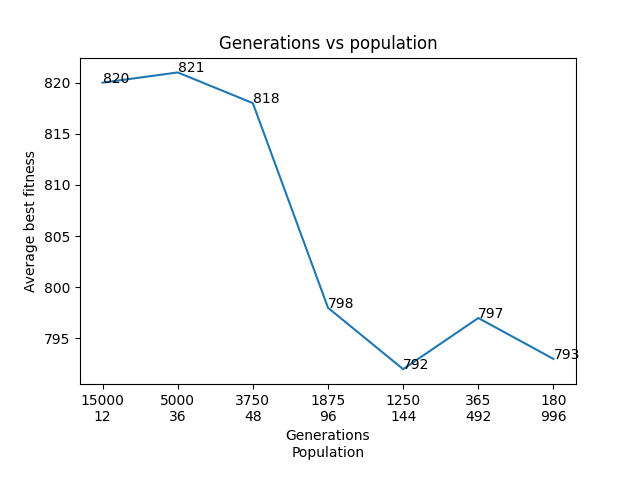
\includegraphics[width=0.6\paperwidth]{generations.png}
    \caption{Výsledky experimentů pro fixní počet vyhodnocení fitness funkce (180~000 vyhodnocení) a proměnlivý počet generací/velikosti populace.}
    \label{gen}
\end{figure}


\end{document}
